\section{Approach}

\cite{Difallah:2012ty}

[MAKE POINT ABOUT ONE OF THE ORIGINAL INTUITION POINTS BEING REDUCING THE ORIGINAL PROBLEM TO AN IMAGE LABELLING PROBLEM, IT'S NOT NECESSARILY OBVIOUS]
[USE \cite{Quinn:2011dj} FOR THE DEFINITION OF THE AGGREGATION PROBLEM]
[HIGHLIGHT HOW, DIFFERENTLY THAN MOST OF CROWDSOURCING IMAGE LABELLING USE CASES, HERE WE'RE COLLECTING TWO LABELS PER "SUBJECT", AND THEY'RE PRACTICALLY INDEPENDENT]
[HIGHLIGHT HOW THE SET OF POSSIBLE VALUES FOR THE LABELS IS NOT LIMITED, IT'S MORE LIKE AN NxN SPACE, N BEING THE SET OF NATURAL NUMBERS, WHERE THE FIRST N REPRESENTS THE ACTUAL NUMBERS 1, 2, 3... AND THE SECOND N THE LETTERS IN THE POSTFIX 1 -> A, 2 -> B, ..., 27 -> AA ...]

\subsection{The social machine mix}

    Although the OLAF data is conceptually simple, assembling such a large dataset as OLAF while assuring sufficient quality still is a complex task.
    
    It is our hypothesis that, to make the best use of pre-existing open data and potentially available technology and human resources, such a problem must be decomposed in a series of complementary sub-problems, each developing parts of its scope and leveraging the peculiarity of its specifications. Each problem, then, can be solved by designing a dedicated socio-technical system, or social machine. This decomposition can take place over several iterations, hence creating a hierarchy of systems that we will call the "social machine mix". 
    
    [THERE SHOULD BE AN IMAGE HERE BUT IMAGE POSITIONING IN LATEX IS TRICKY]

    \begin{figure*}
    	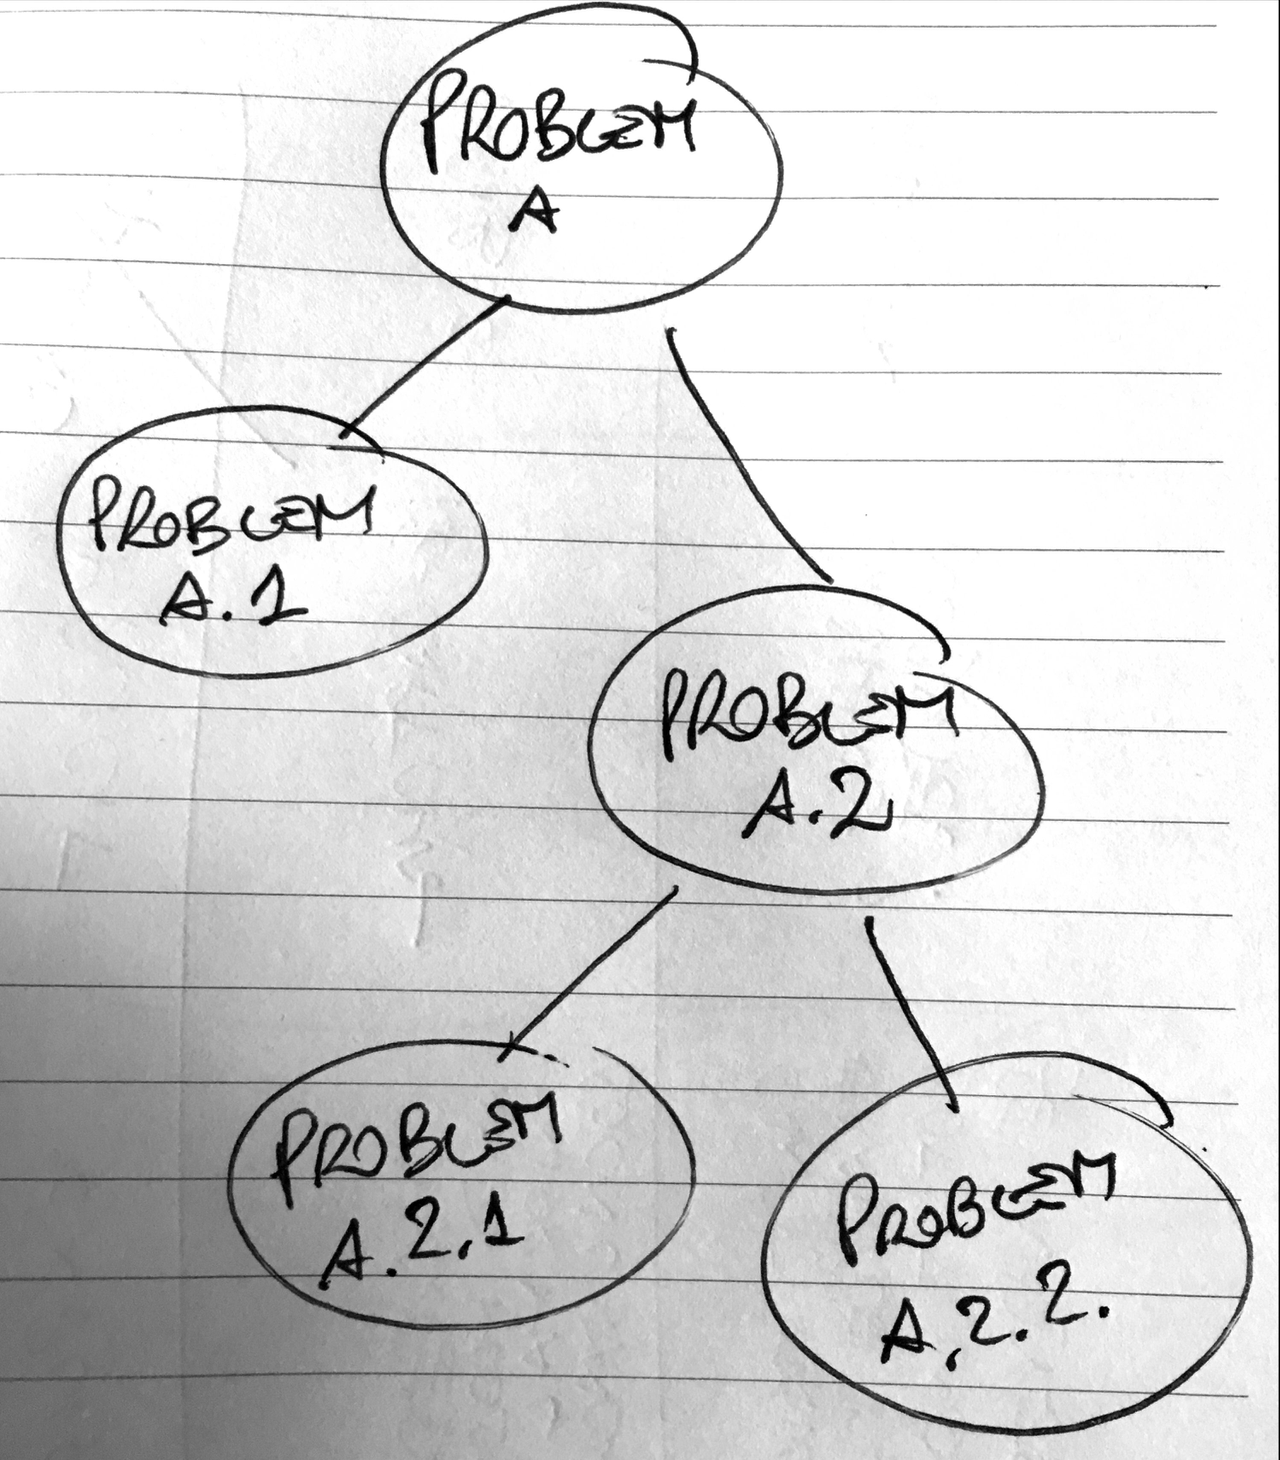
\includegraphics[width=0.95\textwidth]{social-machine-mix-1.png}
    	\caption{This picture should not be here, but apparently it is a nightmare in LaTeX.}
    	\label{fig:social_machine_mix_1}
    \end{figure*}
    
    \textbf{The central role of pre-existing open data.} 
    
    [THIS IS AN INTERESTING STATEMENT, I WONDER IF IT CAN BE GENERALISED] The main driver determining the possible decompositions of the original problem into a hierarchy of sub-problems is the availability of pre-existing and reliable open data. There are two reasons for that.

    \begin{itemize}

        \item The first and more intuitive reason is an assumption: no social machine can produce data in a more effective way than re-using a pre-published, reliable dataset is.  
        
        Hence, re-using existing open data will always be prioritised in respect to re-creating the same, e.g. using crowdsourcing. The focus of social machines in the overall mix should rather be on: a) on creating original data where the same cannot be sourced or computed, and b) on leveraging those skills where humans outperform machines. 
        
        The obvious example of this is using human contributors to survey the streets, being this in person in the physical world, or by examining pictures of the locations, that is how crowdsourcing is used in the system described later in this paper.

        \item The second reason is that open data can be instrumental to operate a social machine. Even when a dataset is not re-used directly to creating the target output data, it can be used for other functions, e.g. supporting the process by which humans contribute. There will be a clear example of this later in this paper. 

    \end{itemize}

\subsection{Scope restrictions}
    
    [DOES NOT SOUND LIKE IN THE RIGHT PLACE, BUT THE SECTIONS THAT COME AFTERWARDS NEED THIS CLARIFICATION BEFORE] 
    
    To make the problem suitable to research it was simplified as described below. 
    
    \textbf{Open data availability.} Although the overarching objective for OLAF is to achieve UK coverage, the availability of open data differs substantially from one UK country to another. Our approach was based on what is available for England and Wales only, as the two have the richer and most homogeneous open data offering, and their territory is estimated to include the 84\% of the 35m addresses in the UK\footnote{[FOOTNOTE EXPLAINING THE ESTIMATE, LIKELY TO BE MADE USING NO. OF HOUSEHOLDS BY COUNTRY FROM ONS AS AN INDICATION OF NO. OF BUILDINGS HENCE ADDRESSES]}.
    
    The validity of the approach is independent of the geographical region that is the subject of the study, as long is the problem is consistent, e.g. the definition of the address is the same. The moment the same open data used for England and Wales becomes available for Scotland and Northern Ireland, the method can be deployed to produce an UK-wide OLAF without modification. Alternatively, if that would not happen, complementary social machines would need being added to the mix.
    
    \textbf{Sample territory.} Within the territory described above, the experiments were performed to address just a sample of the London area, made of five tiles [MORE TECH DESCRIPTION OF WHAT THEY ARE]. This is the same sample that was used in literature in the past to analyse the performance of other geospatial data crowdsourcing initiatives, e.g. OpenStreetMap in [REFERENCE].
    
    \begin{figure*}
    	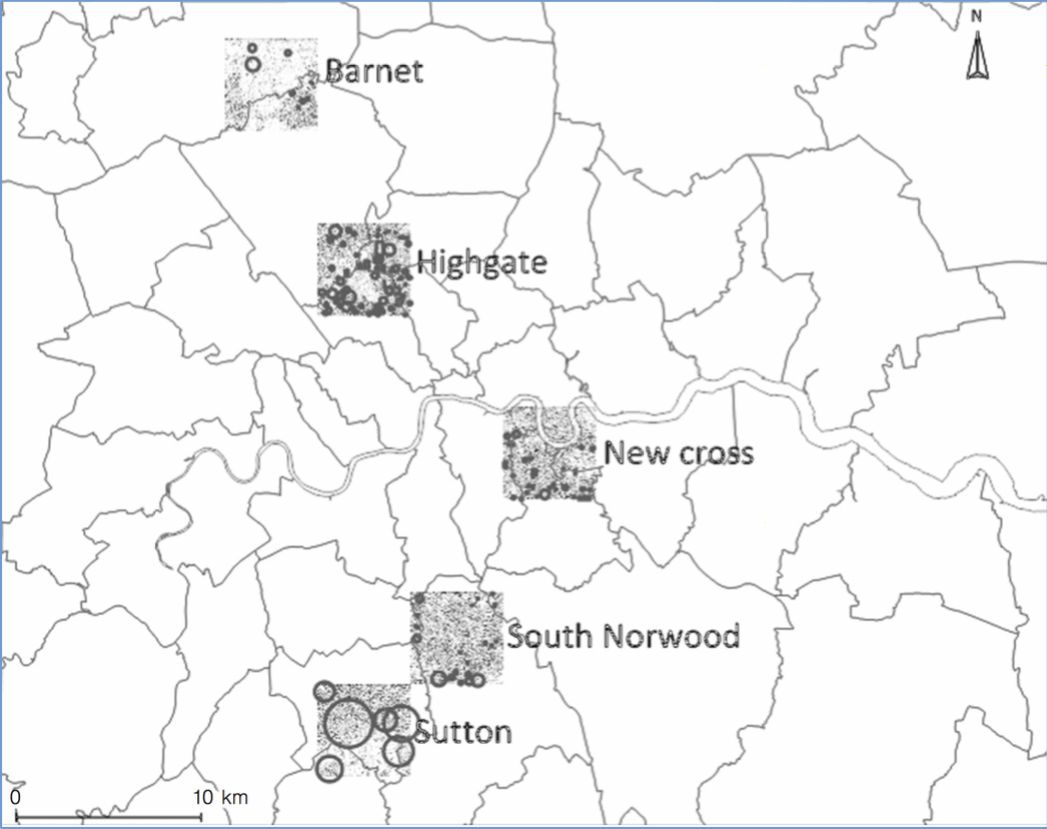
\includegraphics[width=0.95\textwidth]{london-sample-1.png}
    	\caption{This picture should not be here, but apparently it is a nightmare in LaTeX.}
    	\label{fig:london_sample_1}
    \end{figure*}
    
    More precisely, a road is considered in scope if its bounding box, as defined by Ordnance Survey's "Open Names", is completely included in any of the five tiles. 
    
    [SOME WORDING FROM THAT PAPER TO STATE HOW WE DID NOT SIMPLIFY THE PROBLEM BY DOING THIS BUT JUST REDUCED IT IN SIZE].
     
    \textbf{Named vs numbered roads.} Roads that are identified by a number only, e.g. as for motorways, will be considered out of scope.
    
    \textbf{Reliability of the sources.} Only open data from authoritative sources was considered as an option in defining the approach, such as government bodies', and it is assumed to be of the highest possible quality, equivalent to what could be called {\it ground truth}. This allowed the approach not to include any validation of the sources.

\subsection{A social machines mix for OLAF}

    The open data available during our research makes it possible to divide the creation of OLAF in two main sub-problems {\it p1} and {\it p2}. 
    
    \begin{itemize}
        \item {\it p1}: Create a list of all existing {\it house numbers} for each road listed in Ordnance Survey's "Open Names".
        \item {\it p2}: Create a list of all existing {\it house names} for each road listed in Ordnance Survey's "Open Names".
        \item {\it p3}: Create a list of the associations between each of the house number and names above and the list of current\footnote{Postcodes can change. The problem of documenting how addresses change postcode in time is relevant but outside of the scope of research.} postcodes listed in Ordnance Survey's "Open Names". 
    \end{itemize}

    For simplicity, we use the terms "place", "road" and "street" interchangeably, as they are equivalent from a data model perspective in OLAF.

    Open Names "lists definitive place names, roads numbers and postcodes in Great Britain"\footnote{See \url{https://www.ordnancesurvey.co.uk/business-and-government/products/os-open-names.html}.}. It was central to the research work as it is dataset that is functionally closer to the target. OLAF is - in practical terms - equivalent to adding just one dimension to Open Names, that is the list of house names and number for each of its roads. 
    
    Problems {\it p2}\footnote{Note that 98\% of UK addresses are characterised by a house number rather than a house name, so solving {\it p1} is substantially more relevant to achieve completeness in OLAF than {\it p2}.} and {\it p3} are not discussed in this paper. 
    
    Problem {\it p1} can be further decomposed, thanks to the availability of additional open data sources:
    
    \begin{itemize}
        \item {\it p1.1}: Collect the list of house numbers and house names for each existing road as they are referenced in pre-existing open data.
        \item {\it p1.2}: Infer the existence of house numbers from the house numbers collected by {\it p1.1}.
        \item {\it p1.3}: Enable the application of {\it p1.2} by creating the minimum necessary data to trigger more inference.
        \item {\it p1.4}: Correct the output of {\it p1.2}.
    \end{itemize}

    \subsubsection{{\it p1.1}: Collect the list of house numbers and house names for each existing road as they are referenced in pre-existing open data.} 

        References to existing house names and numbers can be found in a few open data publications in the UK. The largest in size is the "Price Paid Data" by the Land Registry (LRPP in the following): a non-ministerial Government department with the responsibility to register the ownership of land and property in England and Wales. Data for each ownership transfer since 1995 - and the full address of the building - is available as open data and updated monthly.
        
        20 years of record make an impressive collection of house names and numbers [MORE ABOUT WHAT THE OUTPUT OF THIS IS]

    \subsubsection{{\it p1.2}: Infer the existence of house numbers from the house numbers collected by {\it p1.1}.} 

        Each culture developed in time a convention for the assignment of house number and names to buildings. In the UK numbering was likely introduced in the early 18th Century as an alternative to house names. Buildings typically are numbered sequentially starting from 1, corresponding to the extremity of the road that is closest to the centre of the town the street is associated to. Odd numbers are on the left-hand side as seen from the centre, even number on the right-hand side. Intermediate properties usually have a number suffixed by one or more letters, this is typical of larger buildings that at some point in time got divided into more smaller dwellings. Modern buildings that have been named by their owner usually retain also a number, that was used by the local government authority during planning.
        
        Centuries of house development and using this system informally of course created many exceptions: e.g. there are buildings for whose house number is zero, places where numbers were assigned consecutively, and house numbers that are simply missing. Simple algorithms, though, have a very high probability to apply the numbering model described above to infer the existence of house numbers from other known house numbers. This is intuitive, as: 
        \begin{itemize}
            \item If we know that one even and one odd house numbers exist in a street, it is likely that all other numbers included within those numbers exist, too (e.g. we can infer 11 and 12 from the existence of 10 and 13)
            \item If we know that two even or odd house numbers exist in a street, it is likely that all other even or odd house numbers included within those numbers exist, too (e.g. we can infer 7 from the existence of 5 and 9, but not 6 and 8, as the right-hand side of the street may not have buildings)
            \item If we know that the same house number in a street is suffixed by two different letters, it is likely that all other letters included within those letters exist, too (e.g. we can infer 14B from the existence of 14A and 14C).
        \end{itemize}
        
        This simple inference is one of the simplest that can be implemented. Other available open data sources enable more complex algorithms, e.g. Ordnance Survey's "Open Maps - Local" [NEED TO CHECK] includes summary shapes for the buildings in each British street, hence enabling the detection of how many buildings are present and suggest how some house numbers may be missing.
        
        {\bf Error in inference.} The described inference criteria add error to the data, made of three components: (i) inferred house numbers that are in reality house names (2) inferred house numbers that in reality exist only in prefixed form instead (e.g. 7A instead of 7), and (iii) addresses that simply do not exist, e.g. because a building was demolished.
        
        We can estimate (i) and (ii) by observing in LRPP. The frequency of addresses identified by a house names instead than a house number is 2\% of the total for the geographic area in scope. This is like saying that 1 out of 50 inferred house numbers was supposed to be a house number instead. The volume of house numbers that exist in prefixed form only instead is [TO CALCULATE, LIKELY INCREDIBLY LOW]. We believe this is an acceptable burden to put on the {\it p1.4} system. 
        
    \subsubsection{{\it p1.3}: Enable the application of {\it p1.2} by creating the minimum necessary data to trigger more inference.} 

        It is clear from the description of problem {\it p1.2} that the inference of house numbers is enabled by the availability of two or more couples of house numbers that act as "seeds" and allow the inference rules to trigger one or more times, for each road.
        
        82\% of the streets in scope are referenced in Land Registry's "Price Paid. The house numbers sourced from {\it p1.1} create opportunities for inference for the 74\% of roads, inferring ~113k house numbers from ~111k known house numbers [DO I NEED TO DESCRIBE THE CALCULATIONS SOMEWHERE IN THE PAPER OR I JUST LINK TO THE GITHUB REPOSITORY WITH THE CODE? THE CODE AT THE MOMENT DOES NOT CALCULATE THE STATISTICS BUT JUST RUNS THE INFERENCE, THIS STUFF WAS CALCULATED 'BY HAND'.]. A substantial number of roads are not described by sufficient data to trigger any inference. 
        
        Because of the above, it suitable to decompose problem {\it p1.3} into two more specialised problems:
        
        \begin{itemize}
            \item {\it p1.3.1}: Enable the application of {\it p1.2} to streets that are not described by pre-existing data.
            \item {\it p1.3.2}: Extend the application of {\it p1.2} beyond the house numbers that are known thanks to pre-existing data.
        \end{itemize}
        
        Problem {\it p1.3.2} is not discussed in this paper. Problem {\it 1.3.1} is about creating the minimum set of data capable of creating the largest sets of inferred house numbers for roads we know nothing of. This means identifying the lowest and highest house numbers for each road for which no house numbers are known\footnote{For simplicity, we did not consider the case where one house number only is known for a street. Those roads are considered as roads with no house numbers.}.

        \begin{figure*}
        	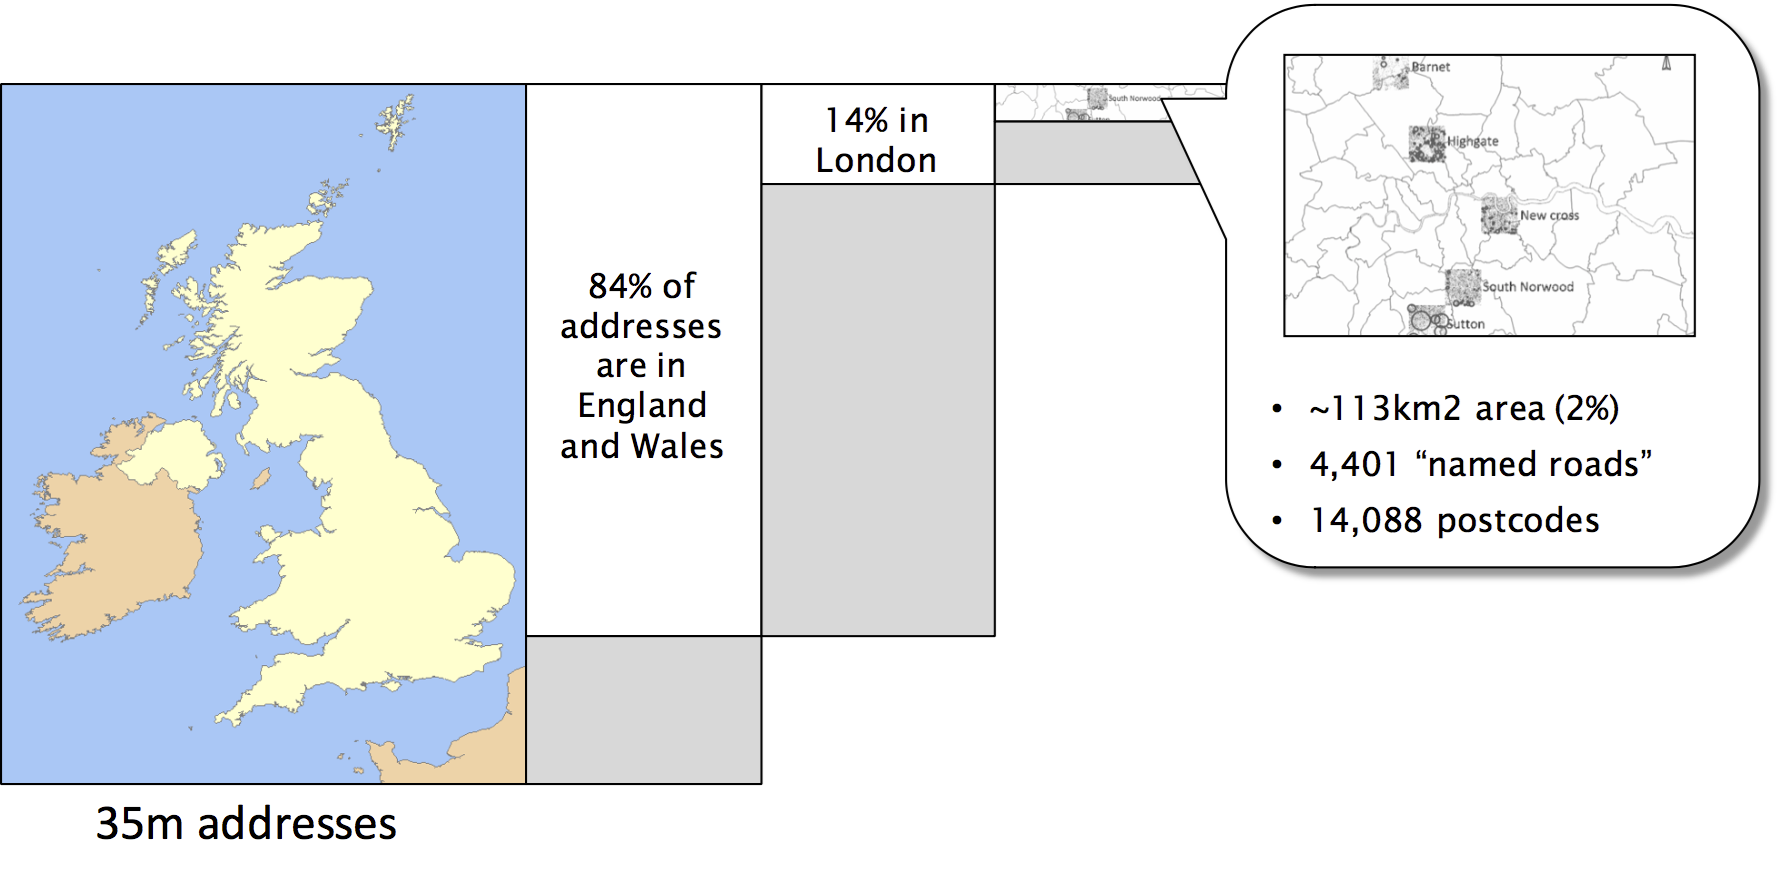
\includegraphics[width=0.95\textwidth]{social-machine-mix-3.png}
        	\caption{This picture should not be here, but apparently it is a nightmare in LaTeX.}
        	\label{fig:social_machine_mix_3}
        \end{figure*}
        
        \begin{figure*}
        	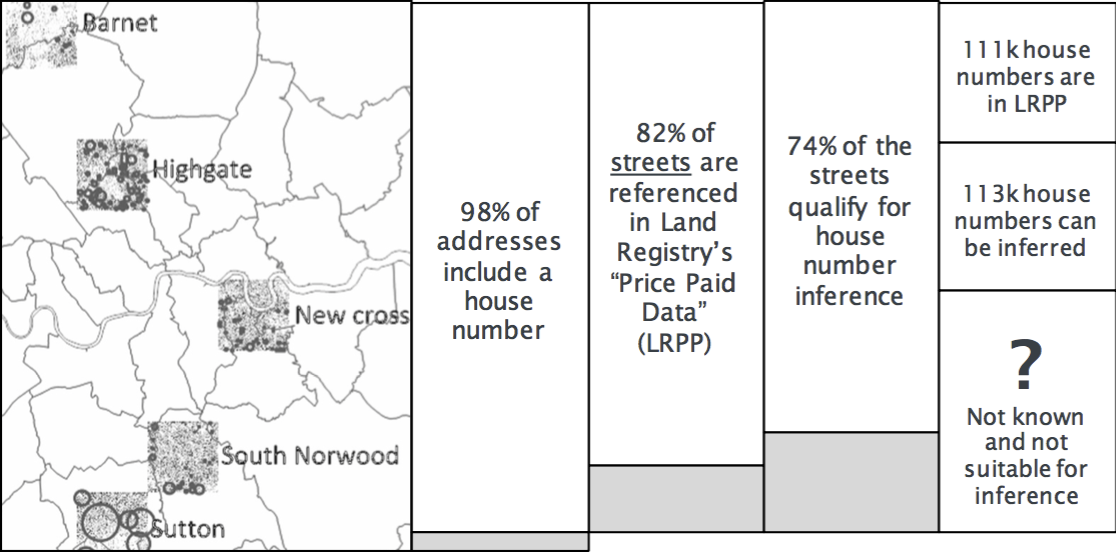
\includegraphics[width=0.95\textwidth]{social-machine-mix-2.png}
        	\caption{This picture should not be here, but apparently it is a nightmare in LaTeX.}
        	\label{fig:social_machine_mix_2}
        \end{figure*}
        
        As no pre-existing open data is available by definition to address this problem, the needed data needs being generated through surveying. 

    \subsubsection{{\it p1.4}: Correct the output of {\it p1.2} through surveying.} 

        Finally, problem {\it p1.4} is about correcting error in {\it p1.2}, typically identifying house numbers that were inferred but do not exist, or that are replaced by house names.
        
        As no pre-existing open data is available by definition to address this problem, the identification of error and the data needed for correction needs being obtained through surveying. 

        Problem {\it p1.4} is not discussed in this paper.

\subsection{Crowdsourcing house numbers to enable inference}

    The focus of the research described in this paper is the solution of problem {\it p1.3.1}. This is not conceptually different than an annotation problem where for each annotated instance there is a single right answer, with a few key differences:
    
    \begin{itemize}
        
        \item For each item subject to annotation, two independent annotations are collected: the lowest and highest visible house numbers. 
        
        There is no use in splitting the task in two, asking one Worker to look for the lowest house number and another to look for the highest. By exploring the pictures of the assigned street the Worker will naturally focus her research on the extremities of the road, where the relevant house numbers are, without knowing in advance which of the two she is finding.
        
        One could argue that the two annotations are not truly independent, as the lowest house number is, by definition, lower than the highest house number. In practical terms, though, the task of surveying a street cannot leverage such mathematical relation. For example, knowing the highest house number won't help the Worker finding the lowest house number, as her finding is rather due toto the observation of the morphology of the street and the progression of nearby house numbers. 
        
        \item The information subject to the annotation could be identified as existing, but the annotation may not be possible anyway. E.g. a Worker will be able to see which the first house in a street is from observing the house numbers on nearby buildings, but vegetation may hide the number. There is also the possibility that Google Street View coverage does not include the surveyed street.
        
        Moreover, unlike other countries, in the UK local authorities do not provide house number plates to the building owners, so this remains their responsibility. Building owners have the option not to affix any plate at all. 
        
        \item There may be nothing to annotate. Because of the nature of the problem, the streets we are using crowdsourcing to collect data about are the ones that appeared little or not at all in pre-existing data, e.g. in Land Registry's Price Paid data over the last 20 years. There likely is a reason for that, e.g. the street may be rural and have few buildings. 
        
    \end{itemize}
    
    The following is a description of the approach that was used for crowdsourcing addresses, that is common to all experimental conditions that were tested.

    \subsubsection{Task model} \leavevmode \\ %% Why is this necessary to get a new line?

        \textbf{Requester.} The Requester desires to gather the lowest and the highest house numbers that can be observed in a specified street, as they can be intelligibly identified by browsing pictures of the street. Alternatively, if no two house numbers are identifiable, the Requester needs being informed, too. Different streets have different degree of interest to the Requester, who is interested in prioritising the collection of the data for the higher interest streets in respect to the lower interest ones. The Requester requires the help of human agents to carry out the tasks, that we will call Workers in the following.
        
        \textbf{Task.} Each HIT (Human Intelligence Task) consists of browsing the pictures of a street until achieving reasonable certainty of having identified the lowest and the highest house numbers or, alternatively, the lack thereof.
        
        \textbf{Strategy.} 
        The strategy relies on traditional crowdsourcing techniques for image labelling.

        \textbf{Crowd $\rightarrow$ Worker.} Each Worker provides judgement on a task by browsing the pictures and declaring if she has found the lowest and the highest house numbers or none. Multiple Workers are asked to identify the house numbers for the same street. The resulting data is chosen through majority voting. We use CrowdFlower as our crowdsourcing platform, presenting each task by embedding customised Google Maps and Google Street View applets into web pages built using the system's templating system. 
    
        \textbf{Quality.} Quality is defined by a combination of (a) accuracy of the Workers in responding to tests questions, and (b) consensus in the data submitted through repeated surveys of the same road. Aggregation takes place accordingly as explained below.
        
    \subsubsection{Workers quality}
    
        Probing Workers using conventional test questions - e.g. where the correspondence of the Worker submissions is checked vs the same data collected by the research team as described in \cite{Kittur:2008gj} - would be a powerful tool to identify high vs low quality Workers, but is very expensive in OLAF's case. The task of surveying a street is not trivial, and early anecdotal evidence showed many Workers leaving after performing no more than two or three surveys. To further damage the performance of the system, the ones who stayed longer started cheating, or showed a substantial drop in their performance. This suggested that spending a substantial part of the Worker's effort on test questions - e.g. making one out of three surveys a test - was not affordable.
        
        Not using any kind of test question is unlikely to be successful, too, and it was explored in previous work such as \cite{DellaPenna:tf} [THIS PAPER ACTUALLY THEORISES THE IMPOSSIBILITY OF GOOD RESULTS WHEN WORKERS HAVE ACCESS TO COMMONLY SHARED PREJUDICE: COULD THIS BE EQUIVALENT TO THE CASE WHERE MY WORKERS ALL END UP BELIEVING THAT SOME EASILY ACCESSIBLE AND VISIBLE CORNER OF A STREET HAS THE HIGHEST HOUSE NUMBER, BUT THE REAL ONE IS ELSEWHERE?]. As an alternative, though, simple test questions can be set up on data that is already available, in a way that is similar to classic anti-spamming techniques like CAPTCHAs as described in \cite{Difallah:2012ty}. In OLAF's case the name of the street itself is used: Workers are asked to copy and paste or type the name of the street as part of their survey. Workers that do not achieve the target accuracy are excluded from further work.

    \subsubsection{Results aggregation}

        Repeated surveys are equivalent to the use of repeated judgement in conventional image labelling exercises. These have been explored extensively in literature and demonstrate that the results produced by a few expensive expert individuals are comparable to what emerges from involving multiple answers by crowds of non-expert Workers, e.g. in \cite{Snow:2008wo} and \cite{Sheng:2008gra}. As the answers are inevitably noisy, different Workers were asked to survey the same road, and their responses are aggregated to decide what is the most likely and truthful observation. 
        
        Approaches to aggregation are an equally well studied subject, and a majority decision is a natural option (e.g. \cite{Le:2010ug}). The detailed parameters and process of how consensus is defined and calculated are tuned for better performance and address issues specific to the context (e.g. in \cite{Hirth:2011fh}). 
        
        In the case of OLAF, consensus is measured by using Fleiss' kappa statistics for inter-annotator agreement, as described for example in \cite{Nowak:2010gt}. For those streets where the house numbers {\it were} stated to be found, a kappa of 60\% on at least 5 surveys is sufficient consensus (e.g. see \cite{Landis:1977kv}). For those streets where the house numbers were stated {\it not} to be found, a kappa of 80\% on at least 10 surveys is required instead, as it is more likely that unreliable Workers agree in reporting that.
        
        The number of 5 and 10 judgements is chosen because they are respectively the minimum number of judgements where 60\% and 80\% kappa can be achieved without the need of an unanimous agreement (4 vs 1 for 60\% and 9 vs 1 for 80\%). 
        
        Rounds of 5 surveys per road are performed until consensus is reached on both its lowest and highest house numbers. Because of the nature of the task, new surveys are performed even if consensus is reached already on either of the two numbers.  
    
    \subsubsection{Recruitment}
        
        We sourced all our Workers from CrowdFlower. For each experiment, we created one dedicated CrowdFlower job. We used identical settings for each experiment set, consisting of the following parameters:
        
        \textbf{Geography} Limited to the top 10 contributor countries in CrowdFlower where English is an official or officially recognised language\footnote{See \url{https://success.crowdflower.com/hc/en-us/articles/202703345-Crowd-Demographics}, the identification of the countries was last repeated on 19 December 2015, before the running the experiments described in this paper. The list of countries is: Bangladesh, Canada, India, Malaysia, Netherlands, Pakistan, Philippines, Sri Lanka, United Kingdom and United States of America.}.
        
        \textbf{Skills} We chose Workers from the default CrowdFlower performance category (formerly named "level 2"), that accounts for 29\% of the total population\footnote{See \url{https://success.crowdflower.com/hc/en-us/articles/202703345-Crowd-Demographics}, the calculation was done on 19 December 2015.}[MORE INTERESTING TO KNOW THE VOLUME OF JUDGEMENTS THEY MAKE, THE OLDER CROWDFLOWER UI SEYI USED GAVE THIS INFORMATION].
        
        \textbf{Accuracy} As described in the previous section, as a test question Workers were asked to copy and paste or type the name of the street as part of their submission in each task. Being the question this simple, error was not accepted the requested accuracy was 99\%\footnote{CrowdFlower does not allow the Requester to set target accuracy to 100\%.}.

        \textbf{Judgements} In groups of 3 per road, repeated until consensus is reached, by different Workers without repetition. Each worker is allowed to contribute to a maximum of 10\% of the streets available to survey at each round.
        
        \textbf{Behaviour} Each Worker was paid for 1 task, and 1 task is made of 1 street to survey.

        \textbf{Reward / Time Limits} The reward was 0.34 US Dollars per task. Workers requiring less than 90 seconds per task were considered at high risk of being malicious and excluded to perform additional tasks. CrowdFlower imposes a time limit of 30 minutes maximum per task[NEED TO CHECK THIS].
    
    \subsubsection{Design}
    \subsubsection{The data processing solution}

        All of the data required to setup the crowdsourcing operation is created from the original distributions by Ordinance Survey and Land Registry. 
        
        The data is stored in a PostgreSQL database\footnote{See \url{http://www.postgresql.org/}.}, that was chosen mostly for its robust and well documented PostGIS extension\footnote{See \url{http://postgis.net/}.}, providing geospatial data processing functionality. NodeJS\footnote{See \url{https://nodejs.org}.} and PostgreSQL scripts were used to import and process the data end to end, up to the point where it is exported to the virtual survey tool, described below. Although the volume of the data being processed is not small, it's far from requiring the tools typical of big data applications. 
        
        The full code is available on GitHub in three repositories:
        
        \begin{itemize}
            \item To import and filter the source Ordnance Survey and Land Registry data in what is then used by the experiments as reference: \url{https://github.com/Digital-Contraptions-Imaginarium/OLAF-yr2_reference_data}
            \item To calculate address inference from the above: \url{https://github.com/Digital-Contraptions-Imaginarium/OLAF-yr2_inference_data}
            \item To consolidate and prepare the data for uploading into the virtual survey tool: \url{https://github.com/Digital-Contraptions-Imaginarium/OLAF-yr2_lab/}.
        \end{itemize}

    \subsubsection{The virtual survey tool}
    
        The virtual survey tool is built exclusively by using the native functionality of two highly available and scalable cloud systems: CrowdFlower and Google Maps and Street View APIs. 
        
        CrowdFlower\footnote{See \url{http://www.crowdflower.com/}.} is a common choice among crowdsourcing services outside of the US\footnote{Differently than Amazon Mechanical Turk, CrowdFlower users are not required to provide an US-registered payment card for registration.}. It offers a full end-to-end solution to run crowdsourcing campaigns, including the recruitment, profiling and management of the Workers, a few tools for quality control, the payment system and the hosting of the actual website through which the Workers contribute. Optionally, some or all of its services can be integrated through APIs into systems owned by its clients. CrowdFlower's particularly suitable to the delivery of open data initiatives as its services are available for free - but for the Workers' compensaton - by choosing their "Data for Everyone" plan, where CrowdFlower reserves the right to publish the data collected through the crowdsourcing jobs. To keep the overall system as simple as possible - while highly scalable and available - it was decided to rely on CrowdFlower's native functionality only and design the system within the limitations of its customisation features.

        The Google Maps and Street View APIs\footnote{See \url{https://developers.google.com/maps/web/}.} allow to embed fully featured interactive maps as part of third party websites. They provide out of the box powerful customisation features through JavaScript scripting, some of which were implemented for the survey tool, such as limiting the user freedom of movement within the maps to the bounding box that contains the street subject to surveying.   
        
        Below is how the tool looks like to a first time user.
    
        \begin{figure*}
        	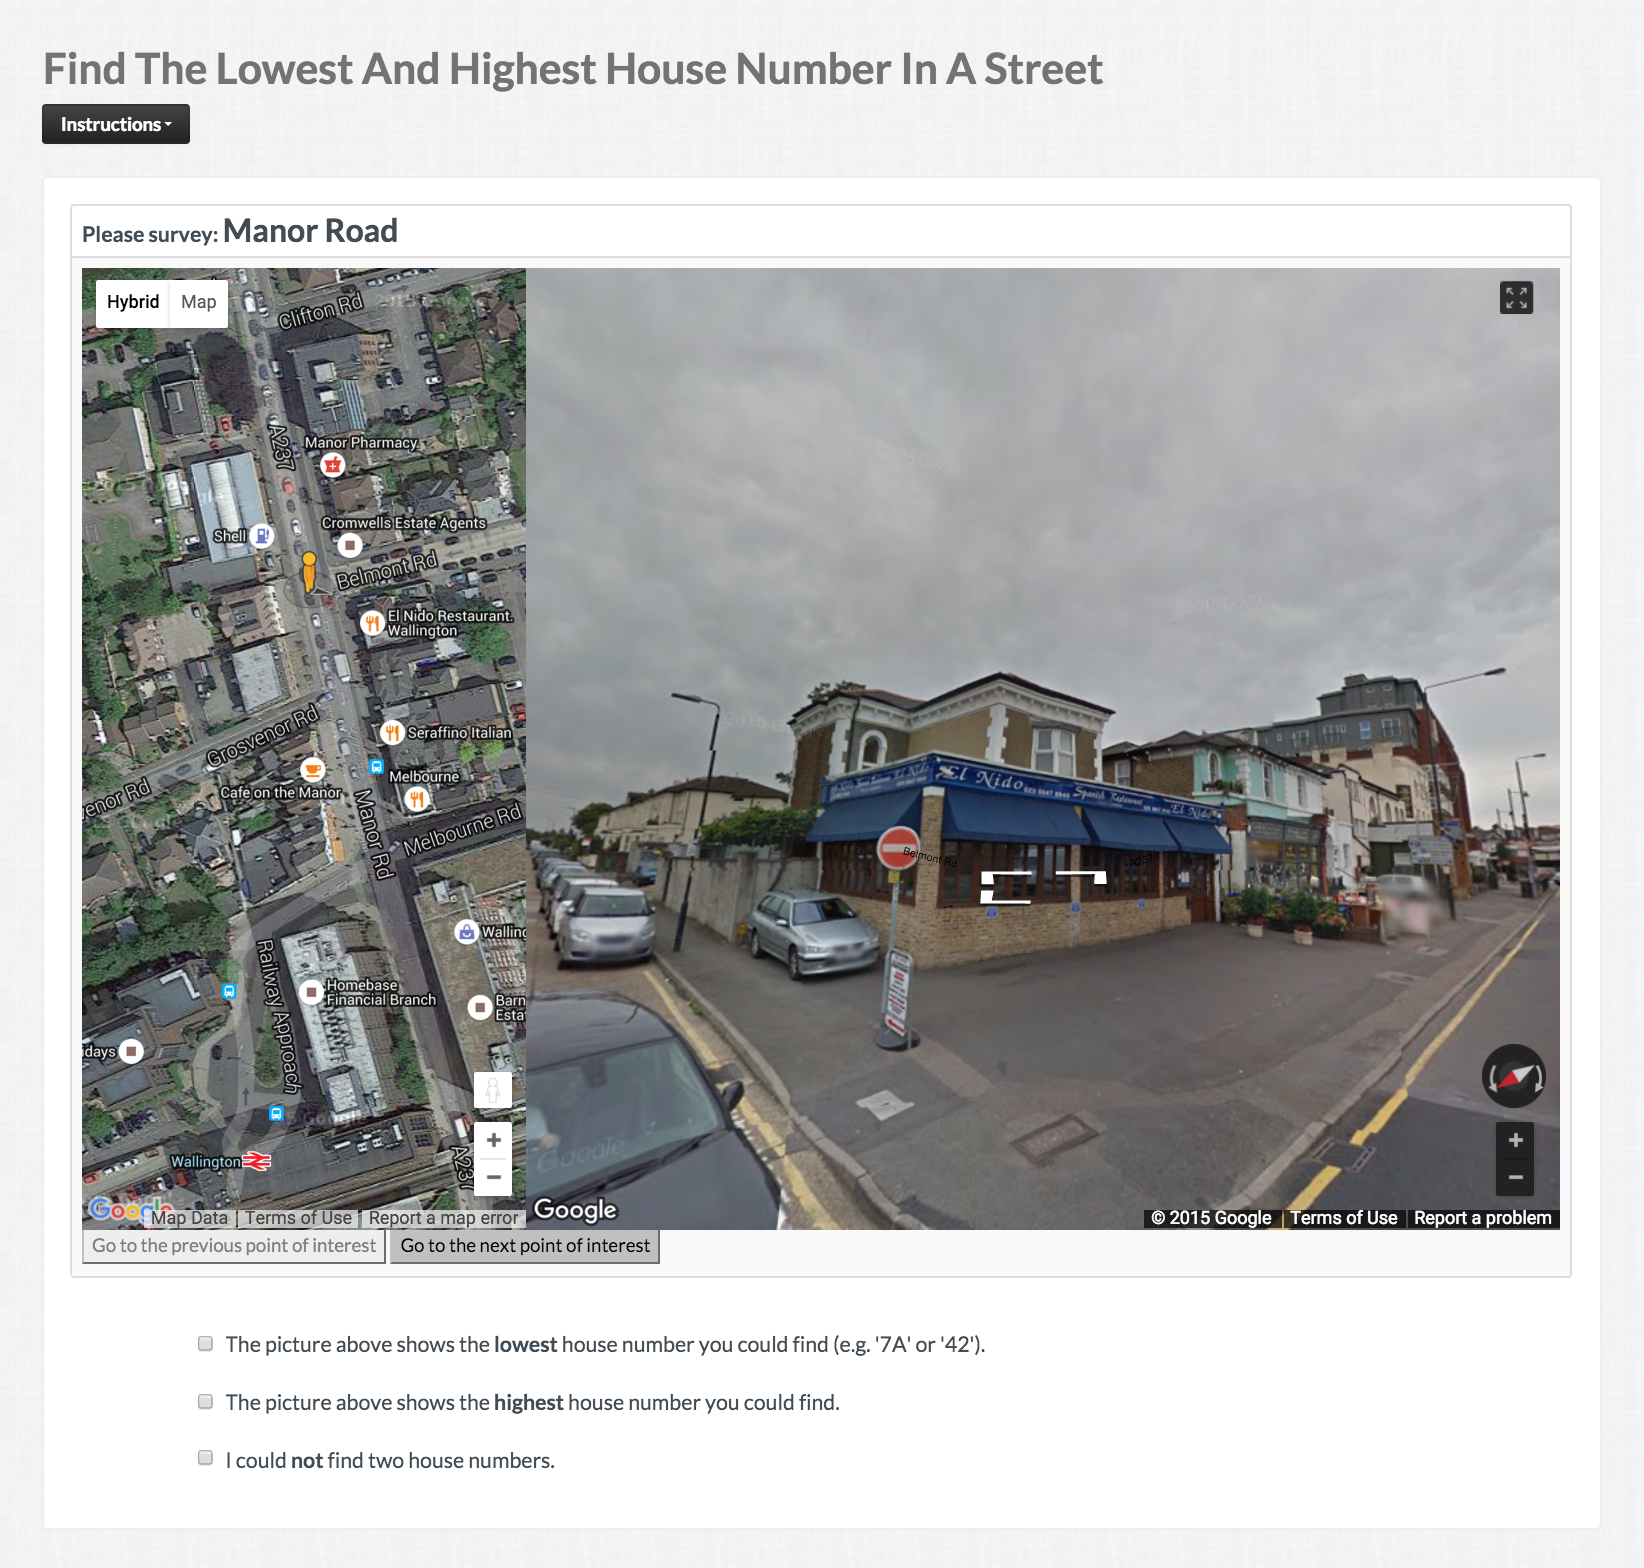
\includegraphics[width=0.95\textwidth]{virtual-survey-tool-01.png}
        	\caption{This picture should not be here, but apparently it is a nightmare in LaTeX.}
        	\label{fig:some_figure}
        \end{figure*}
        
        \paragraph{}

        The full code is available on GitHub at \url{https://github.com/Digital-Contraptions-Imaginarium/OLAF-yr2_lab/}.

    \subsubsection{Legal aspects}

    The choices made to get to the above approach may have legal implications that need to be taken into account, if it was decided to deploy the same methodology in the wild and - in particular - if the data that is the result of the process was published under an open licence, as originally intended. 
    
    To avoid any legal implications of this work, for the time being we are not publishing the data that was collected through our experiments, but just this paper and the source code that was used to build the system. [IS THIS IN CONTRADDICTION WITH THE CHOICE OF CROWDFLOWER'S DATA FOR EVERYONE? MOREOVER, THEIR SYSTEMS ARE NOT IN EUROPE]
    
    What is described below is our early understanding of three of the most interesting legal matters, that would need to be dealt with in future work. 

    \textbf{Personal data and privacy implications.} According to EU Data Protection Directive (95/46/EC\footnote{See \url{http://eur-lex.europa.eu/LexUriServ/LexUriServ.do?uri=CELEX:31995L0046:en:HTML}.} addresses are to be considered "personal data" even when they are not associated to information about who lives at those addresses, as they are "information relating to an identified or {\it identifiable} natural person" (no italics in the original). The directive describes a framework of good practices for member states to make into law that we would need to comply with.
    	
    \textbf{Annotation as derivative work.} Google Maps' terms of service \footnote{See \url{https://www.google.com/intl/en-GB_US/help/terms_maps.html}.} specify a restriction on producing "derivative works of the Content or any part thereof". We believe that asking crowdworkers to examine the Street View pictures and annotate them with the house numbers does not consist in deriving data as it would instead, for example, using a computer vision algorithm to systematically scan the data of pictures, or re-publishing any of machine-readable data that can be retrieved simply by calling Google's APIs. 
    
    \textbf{Database of places.} Again from Google's terms of service comes a restriction on using the services to create "a database of places or other local listings information". We believe that the terms allude to the possibility of re-using Google's data to create a competitor product to any of their services, which is not our case. In general, we also consider addresses as "attributes of places" (e.g. 10 Downing Street, London) rather than "places" (e.g. the UK Prime Minister official residence and office, at 10 Downing Street, London).
    	
    \subsubsection{Scalability}
    
        [THE CALL FOR PAPER EXPLICITLY SAYS THAT "EVIDENCE OF USE IN PRACTICE AND/OR DEMONSTRATION OF SCALABILITY IS REGARDED AS A PLUS"]
    
    \subsubsection{{[}description of additional conditions to test X{]}}
    \subsubsection{{[}description of additional conditions to test Y{]}}

[FIND SOME PLACE TO SAY WHY WE DON'T USE OPENSTREETMAP, BECAUSE SOMEONE WILL ASK. THE ANSWER IS THAT ITS LICENSING IS CONTROVERSIAL ACCORDING TO SOME: E.G. READ \cite{CentreforSpatialLawandPolicy:2014tx}]
    

